%%%%%%%%%%%%%%%%%%%%%%%%%%%%%%%%%%%%%%%%%%%%%%%%%%%%%%%%%%%%%%%%%%
\section{IoT}
\label{sec:iot}

El Internet de las Cosas (del inglés \acrfull{iot}) \cite{iot} \cite{iotamazon} se define como la integración de múltiples sensores o dispositivos físicos interconectados entre sí que se comunican a través de una red inalámbrica y recopilan información en tiempo real. 

\vspace{3mm}

La evolución del \gls{iot} tal y como se conoce en la actualidad tiene sus inicios en los años 90. Sin embargo, en ese entonces estas tecnologías se enfrentaban con la problemática del gran tamaño que presentaban los chips, por lo que se produjo un avance lento de las mismas. A medida que se permitió la reducción del volumen los dispositivos electrónicos y se mejoró la eficiencia y la capacidad de computación de los chips, se facilitó el progreso del \gls{iot}. En los últimos años, la integración de la tecnología 5G o de quinta generación móvil, ha supuesto el incremento de la velocidad de transmisión, procesamiento y análisis de los datos en los sistemas \gls{iot}. La capacidad de administrar a gran escala multitud de dispositivos físicos y la próxima implementación del 6G, depara un futuro en el que las tecnologías \gls{iot} estarán presentes en numerosos ámbitos y sectores.

\vspace{3mm}

Una de las grandes ventajas que proporcionan los sistemas \gls{iot} es la aparición de los entornos \gls{m2m} \cite{m2m}, en los cuales no es necesaria la intervención humana para posibilitar la transmisión y recepción de datos entre los elementos de la red. También, cabe destacar la reducción del coste de computación, la automatización de las tareas y la monitorización en tiempo real. No obstante, en cuanto a posibles desventajas, pueden presentar ciertas vulnerabilidades en cuestiones de privacidad y seguridad. Por ello, en la construcción de un sistema \gls{iot} se deben centrar esfuerzos en blindar los distintos elementos que lo componen frente a posibles ataques que puedan extraer información delicada o sabotear el funcionamiento. En cuanto a la estructura de un sistema \gls{iot}, se pueden diferenciar cuatro componentes que contribuyen al funcionamiento del mismo \cite{iot} \cite{iotamazon}:

\begin{itemize}
    \item Dispositivos inteligentes: Se trata de cualquier elemento físico al que se le pueda asignar una dirección IPv6 y que tenga como mínimo capacidad de computación para recopilar datos del entorno o del usuario y transmitirlos a través de la red. 
    \item Conectividad: En este campo entran varias posibilidades de conexión: Wi-Fi, Bluetooth, redes de área amplia y baja potencia (del inglés \gls{lpwan}) como LoRaWAN, entre otras.
    \item Aplicación: Se compone de un conjunto de servicios de nube que se encargan de integrar y procesar todos los datos recopilados por los dispositivos del sistema \gls{iot}. Además, en algunos ámbitos, emplea técnicas de \gls{ml} para analizar la información que recibe y optimizar la toma de decisiones en el sistema.
    \item Interfaz gráfica: Desde la misma, el usuario puede gestionar y controlar el conjunto de elementos de la red. La interfaz está conectada directamente a la nube y puede tratarse de una aplicación móvil o web.
\end{itemize}

\begin{figure}[h!]
    \centering
    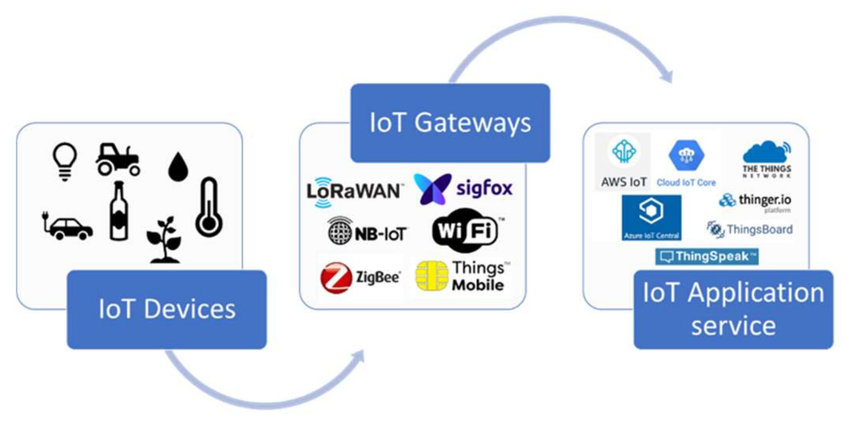
\includegraphics[width=0.8\textwidth]{img/teoria/iot.png}
    \caption{Infraestructura de componentes de un sistema \acrshort{iot} \cite{iotscheme}}
    \label{fig:iot}
\end{figure}

\subsection{IoE}
\label{sec:ioe}

Considerando el contexto energético en el que se engloba este \gls{tfm} y entrando con más detalle en el marco de las tecnologías \gls{iot}, es preciso destacar dentro de las mismas la subcategoría denominada como el Internet de la Energía (del ingles \gls{ioe}) \cite{ioe}. Como concepto, el \gls{ioe} comprende todo el paradigma de operación de los elementos que constituyen una red energética. Es decir, lleva a cabo la integración de todos los dispositivos, sensores o equipos informáticos en una misma estructura, la cual está basada en internet para poder monitorizar y controlar remotamente el estado de cada punto de la red.

\vspace{3mm}
\pagebreak

Se puede expresar que, con la implementación de tecnologías basadas en \gls{ioe}, se buscan objetivos muy similares a las \gls{sg}s. No obstante, el \gls{ioe} va más allá y supone un control y una gestión de la red a mayor escala. En otros términos, no solo se constituye por los elementos de la propia infraestructura eléctrica, sino que también permite una gestión energética a nivel interna de los hogares, mediante la inclusión de electrodomésticos y otros dispositivos electrónicos.


